\documentclass[11pt,a4paper]{article}
\usepackage[T1]{fontenc}
\usepackage[utf8]{inputenc}
\usepackage{lmodern,amsmath,amssymb,graphicx,booktabs,geometry,xcolor,microtype}
\usepackage[round,authoryear]{natbib}
\usepackage{hyperref,fancyhdr,titlesec}
\geometry{left=27mm,right=27mm,top=27mm,bottom=26mm}
\definecolor{forest}{HTML}{173C35}
\definecolor{rust}{HTML}{B44D30}
\hypersetup{colorlinks=true,linkcolor=forest,citecolor=forest,urlcolor=forest,
  pdftitle={When learning changes the match: Information, stability, and exposure in finite markets},
  pdfauthor={},pdfsubject={Research working draft; synthetic matching experiments}}
\titleformat{\section}{\large\bfseries\color{forest}}{\thesection}{.7em}{}
\titleformat{\subsection}{\normalsize\bfseries\color{forest}}{\thesubsection}{.6em}{}
\setlength{\parindent}{1.2em}
\setlength{\parskip}{3pt}
\setlength{\headheight}{14pt}
\pagestyle{fancy}
\fancyhf{}
\fancyhead[L]{\footnotesize\color{forest}INFORMATION, STABILITY, AND EXPOSURE}
\fancyhead[R]{\footnotesize Working paper}
\fancyfoot[L]{\footnotesize\color{gray}Research draft \textbar\ 21 October 2026}
\fancyfoot[R]{\footnotesize\thepage}
\renewcommand{\headrulewidth}{.3pt}
\newtheorem{proposition}{Proposition}
\newtheorem{lemma}{Lemma}
\newenvironment{proof}{\par\noindent\textit{Proof.}\ }{\hfill$\square$\par}
\newcommand{\DA}{\operatorname{DA}}
\newcommand{\IR}{\operatorname{IR}}
\newcommand{\E}{\mathbb{E}}
\newcommand{\ind}{\mathbf{1}}
\newcommand{\BaseLeftMean}{0.0742}
\newcommand{\BaseLeftLow}{0.0658}
\newcommand{\BaseLeftHigh}{0.0827}
\newcommand{\NoiseLeftMean}{0.0090}
\newcommand{\NoiseLeftLow}{0.0033}
\newcommand{\NoiseLeftHigh}{0.0147}
\newcommand{\BudgetLeftMean}{-0.0648}
\newcommand{\BudgetLeftLow}{-0.0705}
\newcommand{\BudgetLeftHigh}{-0.0590}
\newcommand{\BaseRightMean}{0.0743}
\newcommand{\BaseRightLow}{0.0660}
\newcommand{\BaseRightHigh}{0.0828}
\newcommand{\NoiseRightMean}{0.0089}
\newcommand{\NoiseRightLow}{0.0033}
\newcommand{\NoiseRightHigh}{0.0147}
\newcommand{\BudgetRightMean}{-0.0645}
\newcommand{\BudgetRightLow}{-0.0702}
\newcommand{\BudgetRightHigh}{-0.0587}
\newcommand{\ValidationWorlds}{500}
\newcommand{\StressWorlds}{500}
\newcommand{\StressMultiple}{199}
\newcommand{\StressInterior}{15}
\newcommand{\StressLeftLoss}{104}
\newcommand{\EmpiricalPairs}{4184}
\newcommand{\EmpiricalYes}{690}
\newcommand{\EmpiricalPercent}{16.49}


\begin{document}
\thispagestyle{empty}
\begin{flushleft}
{\small\color{forest}\textbf{STABLE MATCHING LAB / RESEARCH WORKING PAPER}}\par\vspace{9pt}
{\LARGE\bfseries\color{forest}When learning changes the match:\par\vspace{4pt}
Information, stability, and exposure\par\vspace{4pt}in finite markets}\par\vspace{9pt}
{\small 21 October 2026 \quad\textbar\quad Theory, exact computation, and independent simulation validation}
\end{flushleft}
\vspace{4pt}
\begin{abstract}
% claim:C008 evidence:P01,N02,N03,N04
Platforms allocate encounters before knowing which pairs will be mutually acceptable. Once an encounter reveals compatibility, requiring stability can change which allocations remain permissible. This paper studies that distinction in finite matching markets. A two-by-two construction with utilities bounded between zero and one shows that a single additional acceptable encounter can make the welfare ratio between unique stable outcomes arbitrarily small. The example concerns mandatory stable reassignment, not the value of information to a planner who may ignore it. An exact decomposition separates unavailable surplus, the stability constraint, and selection of a particular deferred-acceptance outcome. A computational study compares random, score-targeted, and coverage-discounted inspections on identical worlds and budgets. In an independent 500-world baseline validation, coverage raises net surplus by \BaseLeftMean\ per person relative to score targeting; the corresponding adjusted interval is [\BaseLeftLow,\BaseLeftHigh]. A noisier scenario has a smaller positive difference, while increasing inspections can reduce net surplus. Exact small-market benchmarks and a separate selection stress diagnostic distinguish mechanisms that aggregate averages can conceal. A historical encounter-data audit supplies descriptive context without identifying counterfactual policy effects. The results support conditional mechanism comparisons, not a universally optimal scheduler or an empirically calibrated platform recommendation.
\end{abstract}
\noindent\textbf{Keywords:} preference discovery; inspection allocation; cardinal welfare; partial-information stability; simulation validation.

\vspace{7pt}
\noindent\fcolorbox{forest!25}{forest!3}{\parbox{.955\linewidth}{\small
\textbf{Reading guide.} Figure~\ref{fig:revelation} gives the mechanism in two pairs. Equation~\eqref{eq:threegap} separates three sources of loss. Section~\ref{sec:validation} tests selected computational findings on independent worlds. These finite arguments are not asserted to be novel impossibility theorems. This is an AI-assisted working draft; author attribution, human source verification, and venue-specific review remain outstanding.}}

\section{Introduction}
% claim:C001 evidence:E01,E02,E03,E04
Matching requires information that participants often obtain through costly contact. An introduction, interview, or date can reveal whether an apparently promising pair is acceptable to both sides. A platform therefore chooses more than a final matching: it also chooses which opportunities become known. Research on interviews, information acquisition, and recommendations has already made these constraints central to matching design \citep{E01,E02,E03,E04}. The question here is narrower: how does the information graph interact with a requirement that the final allocation respect every revealed blocking pair?

Learning and welfare need not move together under that requirement. A newly revealed pair may prefer one another to their existing partners, yet forming that pair can leave displaced participants with large losses. If those losses cannot be compensated through transfers, stable reassignment may reduce aggregate cardinal surplus. This mechanism is different from an unconstrained planner receiving additional information and retaining the option to ignore it. The latter decision problem keeps the old allocation feasible; the former can make it unstable.

% claim:C002 evidence:E10,E11,E09
Stability and cardinal welfare are established competing objectives. Prior work explicitly studies their welfare trade-offs, including arbitrarily severe losses under general preferences \citep{E10,E11}. Accordingly, this paper does not claim the first welfare impossibility for stable matching. Its analytical role is to expose the graph-expansion mechanism with a bounded-payoff, single-edge construction and then connect that mechanism to benchmarks that can be computed and audited. Deferred acceptance (DA) supplies stable outcomes under strict preferences \citep{E09}; it does not generally maximize a cardinal social objective.

The computational contribution is an equal-budget comparison with explicit information access. Every policy sees the same noisy score matrices, inspects the same number of distinct pairs, and uses the same latent market. Random inspection provides a reference. Score targeting concentrates encounters on high predicted bilateral surplus. Coverage discounting penalizes repeated exposure of the same endpoints. Both DA proposer directions are evaluated, and all unmatched participants remain in the welfare denominator. The policies are fixed heuristics; neither posterior optimality nor incentive compatibility is assumed.

Three layers of evidence are kept separate. Finite proofs establish possibility and accounting results. The original exploratory study supplies broad synthetic comparisons; independently generated worlds evaluate six selected contrasts with adjusted uncertainty intervals. A historical speed-dating audit describes observed choices and graph feasibility. It does not identify utilities, inspection costs, or the effect of a modern exposure policy. This separation allows a limited but testable conclusion: spreading encounters can improve a score-targeted schedule under particular information and market conditions, while learning and spending more need not improve stable net welfare.

\section{Position relative to existing work}
% claim:C003 evidence:E01,E02,E03,E04,E05
\citet{E01} study bilateral interviews that refine preference information and analyze offline interview benchmarks. \citet{E02} examine costly information acquisition and regret-free stability in a many-to-one environment. \citet{E03} combine theory and laboratory evidence to compare information acquisition under centralized mechanisms. \citet{E04} design informative signals and recommendations that reduce communication needed to clear matching markets. These works establish that costly discovery and congestion are substantive prior research areas. The present finite simulation does not reproduce their computational guarantees, equilibrium concepts, or behavioral experiments. Its common-information, common-budget comparison concerns the cardinal outcomes of specified inspection schedules followed by DA. Uncertain-preference stability is likewise a distinct modeling choice rather than a single universal criterion \citep{E05}.

% claim:C004 evidence:E10,E11,E06,E07
The cardinal benchmarks follow the distinction between stable and welfare-oriented allocations emphasized by \citet{E10,E11}. The implemented three-gap computation separates the best stable outcome from a particular proposer-optimal outcome; taking the better of the two DA extremes is not generally sufficient. Exposure is a further objective, informed by work on recommendation fairness \citep{E06}. Coverage discounting has none of that work's allocation guarantees. A dating-platform field experiment also motivates attention congestion \citep{E07}, but does not calibrate the popularity parameter, the inspection cost, or the scheduler evaluated here. These are model assumptions, not estimated behavioral quantities.

These distinctions define a finite comparison of graph-dependent cardinal outcomes under a fixed stability rule. Analytical constructions identify possibilities, exact benchmarks identify the corresponding source of loss, and independent worlds evaluate selected average comparisons. This combination supplies an auditable research object without establishing a new impossibility theorem, a strategic equilibrium, or an empirically superior service.

\section{Model: what is known, revealed, and required}\label{sec:model}
\subsection{Participants, utilities, and inspection graphs}
Let $\mathcal A$ and $\mathcal B$ be finite sets with sizes $n$ and $m$. Left participant $i$ obtains utility $u_{ij}$ from right participant $j$; right participant $j$ obtains $v_{ji}$. Their outside utilities are $r_i$ and $s_j$. A pair is individually rational only if both gains above these outside options are strictly positive. Define the full acceptable graph
\begin{equation}
F=\{(i,j):u_{ij}>r_i,\ v_{ji}>s_j\}.
\end{equation}
A bilateral inspection reveals both utilities on a distinct pair. Let $H\subseteq\mathcal A\times\mathcal B$ be the inspected graph and $B_H=|H|$ its realized inspection count. The acceptable revealed graph is $E=H\cap F$. Inspections that reveal an unacceptable pair still incur cost.

The platform sees noisy scores before choosing $H$, but not the true utilities. After all inspections, participants rank acceptable revealed partners truthfully and can rematch freely. A matching $M\subseteq E$ is stable on $E$ if no pair in $E$ strictly prefers each other to its assigned partners or to being unmatched. This is a revealed-graph requirement; hidden pairs in $F\setminus E$ may still block the allocation under full information. A fixed index refinement resolves ties. The Gaussian experiments have continuous utilities, so exact ties occur with probability zero.

These timing assumptions matter. There are no early binding commitments, strategic reports, endogenous entry decisions, or individual inspection-cap constraints. The final matching is recomputed with all participants available. A real service with irreversible choices or privacy limits would define another mechanism.

\subsection{Welfare and references}
The outside-relative gross surplus of a matching is
\begin{equation}\label{eq:surplus}
S(M)=\sum_{(i,j)\in M}\left[(u_{ij}-r_i)+(v_{ji}-s_j)\right].
\end{equation}
Unmatched participants contribute zero incremental surplus. Summing these nontransferable utilities assumes a common cardinal scale; it does not make compensation possible. With nonnegative per-pair inspection cost $c$, net surplus per person is
\begin{equation}\label{eq:net}
W(H;c)=\frac{S(M_E)-c|H|}{n+m}.
\end{equation}
The cost is an aggregate platform burden. It is not subtracted from participant-specific utilities when reporting their Gini coefficient or side means.

Write $\mathcal M(E)$ for all individually rational matchings on $E$, and $\mathcal S(E)\subseteq\mathcal M(E)$ for stable matchings under the fixed strict preferences. For proposing side $p\in\{L,R\}$, define
\begin{align}
P(F)&=\max_{M\in\mathcal M(F)}S(M),&
P(E)&=\max_{M\in\mathcal M(E)}S(M),\\
T(E)&=\max_{M\in\mathcal S(E)}S(M),&
D^p(E)&=S(\DA^p(E)).
\end{align}
The full planner $P(F)$ is a free-information diagnostic bound, not an implementable equal-budget competitor. The revealed planner $P(E)$ need not be stable. The best stable value $T(E)$ can exceed both DA extremes; the exact solver searches the stable set rather than assuming one extreme maximizes total surplus.

\section{Analysis: three mechanisms that averages can hide}\label{sec:analysis}
\subsection{One encounter can remove almost all stable welfare}
The following construction gives the mechanism with bounded utilities and unique stable outcomes. Its role is explanatory and diagnostic, not a claim of priority over established cardinal stability losses.

% claim:C009 evidence:P01
\begin{proposition}[Vanishing retention under graph expansion]\label{prop:ratio}
For every $\eta>0$, there is a two-by-two market with all utilities in $[0,1]$ and inspected acceptable graphs $E\subset F$ differing by one edge, such that each graph has a unique stable matching and
\begin{equation}
\frac{D^p(F)}{D^p(E)}<\eta
\end{equation}
for either proposing side. The number of matched pairs falls from two to one.
\end{proposition}

\begin{proof}
Choose $0<\varepsilon<1/2$ such that $2\varepsilon/(1+\varepsilon)<\eta$. Outside utilities are zero. Matrices $U$ and $V$ list utilities by left and right rows, respectively:
\begin{equation}\label{eq:witness}
U=\begin{pmatrix}\varepsilon&2\varepsilon\\0&1\end{pmatrix},\qquad
V=\begin{pmatrix}1&0\\2\varepsilon&\varepsilon\end{pmatrix}.
\end{equation}
On $E=\{(0,0),(1,1)\}$, stability requires both diagonal pairs, giving surplus $2+2\varepsilon$. Reveal $(0,1)$ to obtain the full acceptable graph $F$. Participants $a_0$ and $b_1$ strictly prefer each other to any alternative, so any stable matching must contain their pair. The remaining participants have no acceptable edge. The unique stable surplus is $4\varepsilon$, and the ratio is $2\varepsilon/(1+\varepsilon)\to0$.
\end{proof}

\begin{figure}[tbp]
\centering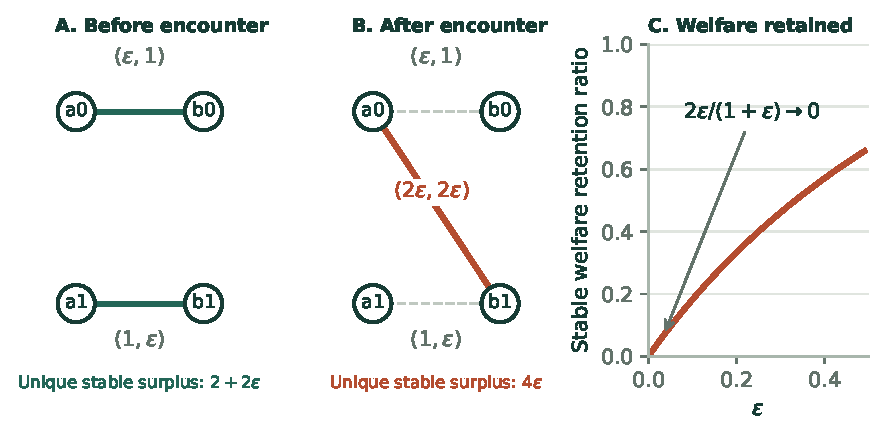
\includegraphics[width=\linewidth]{generated/revelation.pdf}
\caption{A single encounter changes the stability requirement. Payoff pairs list left and right utilities. Solid lines are matched; dashed diagonal edges remain acceptable but are not selected. The added pair gains only $\varepsilon$ per endpoint relative to the diagonal outcome, while displacing two participants who each lose utility one. Panel C plots the exact retention ratio, not simulated observations. All utilities lie in $[0,1]$.}\label{fig:revelation}
\end{figure}

The unrestricted planner can keep the diagonal allocation even after learning the extra edge. Its feasible set expands, so its maximum cannot fall. The stable mechanism instead acquires an additional blocking constraint. Proposition~\ref{prop:ratio} concerns that changing constraint, not a negative information value for a decision maker allowed to disregard the signal. It gives an arbitrarily small multiplicative ratio, not an unbounded additive loss with bounded payoffs.

\subsection{Information, stability, and outcome selection}
% claim:C010 evidence:P01,N01
\begin{proposition}[Three-gap identity]\label{prop:gaps}
For every revealed graph and either proposing side,
\begin{equation}\label{eq:threegap}
\underbrace{P(F)-D^p(E)}_{\text{total gross shortfall}}
=\underbrace{P(F)-P(E)}_{I(E):\ \text{information}}
+\underbrace{P(E)-T(E)}_{C(E):\ \text{stability constraint}}
+\underbrace{T(E)-D^p(E)}_{Q^p(E):\ \text{DA selection}},
\end{equation}
and all three components are nonnegative.
\end{proposition}
\begin{proof}
Matchings on $E$ are feasible on $F$, stable matchings on $E$ are feasible matchings on $E$, and DA returns one stable matching. Thus $P(F)\ge P(E)\ge T(E)\ge D^p(E)$. The identity follows by telescoping.
\end{proof}

The distinction is substantive even though the algebra is elementary. In Proposition~\ref{prop:ratio}, full revelation leaves a unique stable outcome, so the entire planner shortfall is a stability constraint and $Q^p(F)=0$. Conversely, take complete acceptable preferences with
\begin{equation}\label{eq:selection}
U=\begin{pmatrix}3&2\\2&3\end{pmatrix},\qquad
V=\begin{pmatrix}1&100\\100&1\end{pmatrix}.
\end{equation}
Left-proposing DA chooses the diagonal, with surplus eight. The off-diagonal allocation is also stable and gives surplus 204, attaining the unrestricted planner optimum. Here the pure stability gap is zero and the DA-selection gap is 196. This separate example uses a different utility scale and is not pooled with the bounded construction or the Gaussian experiments.

Relative to the gross full planner, the net shortfall adds $c|H|$ to the three terms. With identical realized inspection counts, the cost cancels from policy contrasts. With different counts, subtracting $c(|H_1|-|H_2|)$ is essential. The old two-term allocation gap $P(E)-D^p(E)$ merges $C(E)$ and $Q^p(E)$ and cannot identify either separately.

\subsection{What higher inspection costs do imply}
Nonmonotone gross DA welfare does not prevent a useful cost comparative static. Fix a finite set of schedules $q$, each with expected gross surplus $G_q$ and expected inspection count $B_q$. Their distributions and final matching rules are held fixed as $c$ changes. Include zero inspections if abstention is available.

% claim:C011 evidence:P01
\begin{proposition}[Finite-schedule cost envelope]\label{prop:cost}
The value $V(c)=\max_q\{G_q-cB_q\}$ is continuous, convex, piecewise linear, and nonincreasing for $c\ge0$. An optimal budget, with smaller-budget tie-breaking, is weakly decreasing in $c$.
\end{proposition}
\begin{proof}
The maximum of finitely many nonincreasing affine functions has the stated value properties. At $c_1<c_2$, let optimal schedules have $(G_1,B_1)$ and $(G_2,B_2)$. Optimality gives $G_1-c_1B_1\ge G_2-c_1B_2$ and $G_2-c_2B_2\ge G_1-c_2B_1$. Adding yields $(c_2-c_1)(B_1-B_2)\ge0$, hence $B_1\ge B_2$.
\end{proof}

For two candidates with $B_b>B_a$, the higher budget is weakly preferred precisely when $c\le(G_b-G_a)/(B_b-B_a)$. Such pairwise thresholds need not be breakpoints of the optimized envelope if another schedule dominates. The result optimizes only the stated candidate set. It neither proves a globally optimal acquisition policy nor removes selection bias when schedules are chosen and evaluated on the same noisy worlds.

\section{Computational design}\label{sec:design}
\subsection{A shared synthetic information environment}
Draw independent standard-normal popularity terms $A_i,B_j$ and pair shocks $X_{ij},Z_{ij}$. Parameters satisfy $\alpha\in[0,1]$, $\rho\in[-1,1]$, and $\sigma\ge0$. Utilities are
\begin{align}\label{eq:dgp}
u_{ij}&=\sqrt\alpha\, B_j+\sqrt{1-\alpha}\,X_{ij},\\
v_{ji}&=\sqrt\alpha\, A_i+\sqrt{1-\alpha}\left(\rho X_{ij}+\sqrt{1-\rho^2}Z_{ij}\right).
\end{align}
Each marginal utility has variance one. Shared popularity correlates different participants' evaluations of a common partner. The reciprocal utility correlation on a pair is $(1-\alpha)\rho$, so varying $\alpha$ also changes that correlation. The parameter is not an isolated causal congestion treatment. Observable scores are $\hat u_{ij}=u_{ij}+\sigma\xi_{ij}$ and $\hat v_{ji}=v_{ji}+\sigma\zeta_{ij}$ with independent standard-normal noise. They are signals, not posterior expected utilities. Full score matrices are free to the scheduler; screening costs are excluded.

Let predicted surplus above the outside option be $a_{ij}=\hat u_{ij}-r_i$ and $b_{ji}=\hat v_{ji}-s_j$. Score greedy ranks
\begin{equation}
z_{ij}=(a_{ij}^{+}+b_{ji}^{+})\ind\{a_{ij}>0,b_{ji}>0\}.
\end{equation}
Coverage chooses successive uninspected edges maximizing
\begin{equation}\label{eq:coverage}
\frac{z_{ij}+10^{-6}}{[(1+d_i)(1+d_j)]^\gamma},\qquad \gamma=1,
\end{equation}
where $d_i,d_j$ count allocated inspections. The small floor gives zero-score pairs a coverage tie rule. The schedule updates endpoint degrees, not beliefs from newly inspected utilities. Random chooses a uniform set of distinct pairs. Every policy inspects exactly $\min(B,nm)$ pairs, then DA is run on revealed acceptable edges.

The baseline has 24 participants per side, $\alpha=.5$, $\rho=.5$, $\sigma=1$, zero outside utilities, and $c=.05$. The original eight scenarios additionally cross low/high popularity with precise/noisy scores, use negative reciprocity, halve the right side, or assign half of each side outside utility .75. Four budgets are $24,48,96,192$. Per scenario, 100 world draws are paired across three policies, four budgets, and both proposer directions, yielding 19,200 treatment rows. These are not 19,200 independent observations. Seeds also recur across scenarios; comparisons condition on scenario. Random inspection sets are not constrained to be nested across budgets.

Outcomes include whole-population net surplus, fraction matched, each side's mean surplus, minimum side exposure rate, gross-surplus Gini, and full latent blocking density. Exposure means at least one inspection, not a successful match or protected-group fairness. Revealed blocking is checked to be zero. Global blocking is observable to the synthetic analyst only because true uninspected utilities are available for evaluation, not scheduling.

\subsection{Exact references and validation samples}
The original 30 eight-by-eight worlds provide 540 small-market treatment rows. An exact dynamic program computes unrestricted planner surplus on full and revealed graphs. To compute $T(E)$, the exact stable solver uses the invariant set of matched participants under strict one-to-one stable matching (Appendix~\ref{app:matched}) and enumerates every bijection between those matched sets. With $k\le8$ matched pairs, at most $k!$ candidates are examined; unacceptable assignments and blocking pairs are rejected. Independent tests brute-force all partial matchings on tiny rectangular and tied instances without assuming that reduction.

No positive DA-selection gap was found in those original rows. A separate, explicitly post hoc diagnostic therefore uses 500 complete four-by-four markets with independent $U(.1,10)$ utilities. Its scale and acceptability differ from the Gaussian experiment. The diagnostic checks that the exact benchmark can distinguish stable outcome selection when competing stable allocations occur. It is not pooled with the primary study or called an independent replication of its data-generating process.

For selected synthetic claims, new seeds generate 500 independent worlds within each of the baseline and high-popularity/noisy scenarios. Seeds recur across scenarios, so their estimates can be correlated; Bonferroni adjustment does not require those comparisons to be independent. Policies remain untuned. Six primary contrasts consist of coverage versus greedy at budget 48 in each scenario, and coverage budget 192 versus 96 in the baseline, for each proposer side. Whole-world paired bootstrap uses 20,000 draws. Alongside ordinary 95\% intervals, the paper reports nominal marginal 99.1667\% intervals from a Bonferroni adjustment over six contrasts. Bootstrap coverage and the resulting family-wise interpretation are approximate, not exact finite-sample guarantees. The contrast plan was recorded before these new worlds were executed, after the original exploratory results were known; it was not externally preregistered.

\clearpage
\section{Results: conditional gains and separate sources of loss}\label{sec:validation}
\subsection{Independent worlds support a smaller effect under noisier scores}
Table~\ref{tab:validation} and Figure~\ref{fig:validation} report all six validation contrasts. In the baseline, the coverage advantage is about .074 surplus units per person for either proposer side. The adjusted left-proposing interval is [\BaseLeftLow,\BaseLeftHigh]. The high-popularity/noisy difference is much smaller: \NoiseLeftMean\, with adjusted interval [\NoiseLeftLow,\NoiseLeftHigh]. In the original 100-world exploration its interval crossed zero. The larger independent sample supports a small positive difference; it would be incorrect to preserve the earlier imprecision as evidence of no effect.

\begin{table}[tbp]
\centering\small
\caption{Independent synthetic validation. Entries are paired net-surplus differences per person, not percentages. All six planned contrasts are retained. Adjusted percentile intervals have nominal marginal coverage 99.1667\%; resampling unit is the world.}\label{tab:validation}
\begin{tabular}{llrr}\toprule
Contrast & Proposer & Mean & Adjusted interval \\\midrule
Baseline policy & Left & 0.0742 & [0.0658, 0.0827] \\
Noisy/popular policy & Left & 0.0090 & [0.0033, 0.0147] \\
Budget 192 minus 96 & Left & -0.0648 & [-0.0705, -0.0590] \\
Baseline policy & Right & 0.0743 & [0.0660, 0.0828] \\
Noisy/popular policy & Right & 0.0089 & [0.0033, 0.0147] \\
Budget 192 minus 96 & Right & -0.0645 & [-0.0702, -0.0587] \\
\bottomrule\end{tabular}

\end{table}

\begin{figure}[tbp]
\centering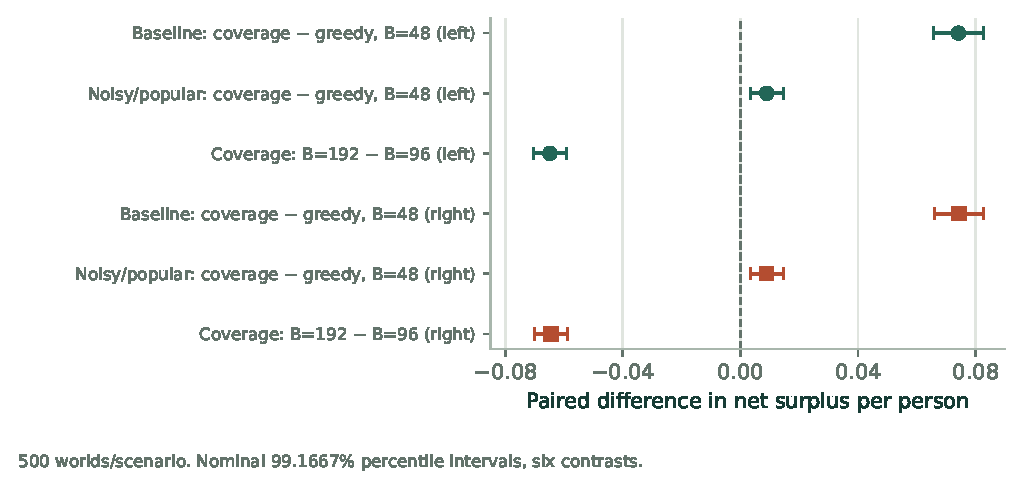
\includegraphics[width=\linewidth]{generated/validation.pdf}
\caption{Policy and budget contrasts on 500 new worlds per scenario. Circles denote left-proposing DA; squares denote right-proposing DA. Intervals are Bonferroni-adjusted percentile bootstrap intervals over six comparisons. The schedule family and structural parameters are held fixed.}\label{fig:validation}
\end{figure}

The results do not establish coverage's global dominance. The original exploration retained a slightly negative mean difference in the scarce-right, large-budget case, with an interval spanning zero. Independent validation covers only the selected scenarios and budgets. Coverage's mechanism also differs from a fully Bayesian acquisition policy: an endpoint exposure penalty can improve diversity of opportunity without being optimal for information value.

\subsection{More inspections can lower net surplus despite more matching}
The validation budget contrast compares the same coverage rule at 192 and 96 inspections. The left-proposing net-surplus difference is \BudgetLeftMean\ per person, with adjusted interval [\BudgetLeftLow,\BudgetLeftHigh]; right-proposing results are similar. This supports a cost-adjusted comparison at the chosen $c=.05$, not a universal negative gross value of information or proof that 96 is the optimal budget. The analytic graph-expansion example establishes a different claim: gross stable surplus can fall even before inspection costs.

Figure~\ref{fig:cost} shows the finite-schedule cost envelope on training means. Budgets for six cost values are selected using the original worlds, frozen, and then evaluated on new worlds in Table~\ref{tab:cost}. At zero cost the training choice is 192 inspections; at cost .05 it is 96; at cost .1 it is 48. These choices satisfy Proposition~\ref{prop:cost} within the candidate set. They are not optimal meeting counts for a real population.

\begin{figure}[tbp]
\centering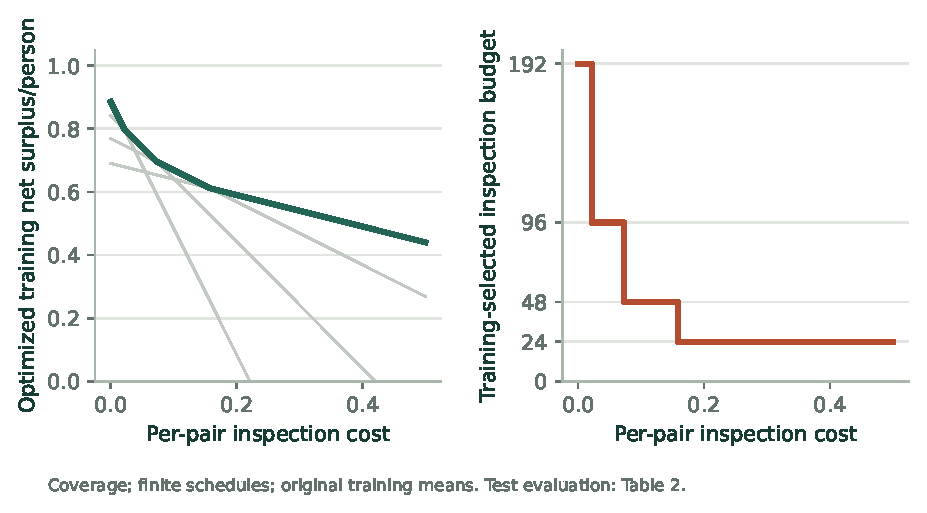
\includegraphics[width=\linewidth]{generated/cost_envelope.pdf}
\caption{Cost changes the choice among fixed inspection schedules. Left: the upper envelope of training mean net-surplus lines. Right: the associated budget with smaller-budget tie-breaking. Coverage schedules and the zero-inspection option form a finite candidate set; no new schedule is optimized for each cost.}\label{fig:cost}
\end{figure}

\begin{table}[tbp]
\centering\small
\caption{Training-selected coverage budgets evaluated on held-out baseline worlds, left proposer. Intervals are ordinary 95\% world-bootstrap intervals conditional on the frozen training choice; they are descriptive secondary comparisons.}\label{tab:cost}
\begin{tabular}{rrrr}\toprule
Cost per pair & Selected budget & Test net/person & 95\% interval \\\midrule
0.000 & 192 & 0.8782 & [0.8686, 0.8880] \\
0.025 & 96 & 0.7930 & [0.7833, 0.8028] \\
0.050 & 96 & 0.7430 & [0.7333, 0.7528] \\
0.100 & 48 & 0.6678 & [0.6582, 0.6774] \\
0.200 & 24 & 0.5924 & [0.5816, 0.6033] \\
0.400 & 24 & 0.4924 & [0.4816, 0.5033] \\
\bottomrule\end{tabular}

\end{table}

\subsection{The exact benchmark identifies what did not happen}
Figure~\ref{fig:gaps} decomposes the original small-market shortfall. All 540 rows have numerically zero DA-selection loss, within the implementation tolerance. Accordingly, their previous combined allocation gap is attributable to the stability constraint on those realized graphs. This is a sample-specific result; it does not validate replacing the best stable benchmark by DA in arbitrary markets.

\begin{figure}[tbp]
\centering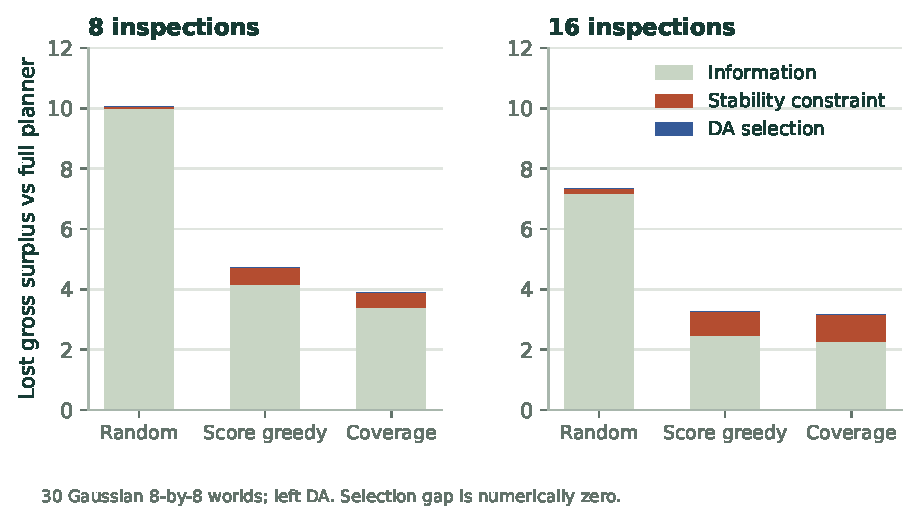
\includegraphics[width=\linewidth]{generated/three_gaps.pdf}
\caption{Exact three-gap accounting on the original Gaussian small markets. Bars show descriptive means, not inferential intervals. No positive selection gap was observed in any of the 540 rows, for either proposer. The information and stability components remain distinct.}\label{fig:gaps}
\end{figure}

% claim:C005 evidence:N03
The separate complete-market diagnostic makes the distinction visible. DA extremes differ in \StressMultiple\ of \StressWorlds\ worlds. The best stable value exceeds left-proposing DA in \StressLeftLoss\ worlds and strictly exceeds both DA extremes in \StressInterior\ worlds. Thus even selecting the better proposer direction can miss the welfare-best stable allocation. These counts validate the benchmark's usefulness in another synthetic population; they do not estimate the frequency of selection losses in the baseline model or in actual dating markets.

\section{Observed encounters: a descriptive bridge, not policy identification}\label{sec:empirical}
% claim:C006 evidence:E08,C02,N04
The original Columbia speed-dating file and dictionary were retrieved and checked locally.\footnote{Original \href{https://www.stat.columbia.edu/~gelman/arm/examples/speed.dating/Speed\%20Dating\%20Data.csv}{CSV} and \href{https://www.stat.columbia.edu/~gelman/arm/examples/speed.dating/Speed\%20Dating\%20Data\%20Key.doc}{data dictionary}, accessed 21 October 2026. Retrieval details and file hash accompany the aggregate audit.} After excluding ten unusable directed rows and deduplicating reciprocal records, the audit contains \EmpiricalPairs\ encounters across 21 waves, with \EmpiricalYes\ mutual-yes edges (\EmpiricalPercent\%). All represented within-wave cross-side pairs are observed. This is more complete than a selective recommendation log, but does not establish complete capture of every recruited participant. Resampling whole waves gives a descriptive 95\% interval of 14.93--18.27\%; heterogeneous waves are not a representative random sample of a modern platform.

% claim:C007 evidence:E08,C02,N04
The dictionary identifies ratings as post-encounter measurements and flags an acceptance-budget wave, an undergraduate wave, different hosts, and book or magazine conditions. Excluding the acceptance-budget wave yields 16.78\% mutual yes; excluding all dictionary-flagged variants yields 16.76\% over 13 waves. These are exploratory sample-composition checks. The acceptance budget limits yes decisions, not the number of inspections. The original paper used 14 sessions \citep{E08}; the all-wave audit is not its estimation-sample replication.

Binary choices do not identify strict rankings, comparable lifetime utilities, outside values, or meeting costs. A maximum of 204 disjoint pairs can be selected on the recorded mutual-yes graphs under an imposed one-to-one restriction, but this is a retrospective feasibility count, not an observed relationship outcome or stable matching estimate. Post-encounter ratings cannot be used as first-encounter scheduling signals without leakage. The analysis therefore neither fits the Gaussian cardinal model nor evaluates counterfactual exposure policies. Only aggregates and source hashes are redistributed; raw individual records remain local.

\section{Discussion and research limits}
The analytical mechanism is a change in admissibility, not a general indictment of learning. When every acceptable discovered pair can block a previous allocation, additional information can add a social constraint. The small private gains of a new pair need not internalize the losses imposed on displaced participants. An institution that can ignore recommendations, permit compensation, bind early commitments, or redefine admissible blocking would face a different problem. The relevant institutional question is which of these assumptions actually applies.

The computations suggest that concentrating encounters on noisy predicted surplus can leave feasible gains undiscovered, and that a simple exposure discount can recover some of them. The independent validation supports this conditional comparison and also shows why a small effect should not be equated with no effect. None of this establishes optimal information acquisition. Screening is free in the model, scores are exogenously supplied, participants do not choose entry, and inspections have no personal degree caps or temporal congestion. Popularity and reciprocal correlation also interact in the data-generating process. These choices define the interpretation rather than disappearing under larger simulation samples.

The exact decomposition sharpens the next research question. An information gap calls for better discovery; a stability gap raises an objective or institutional trade-off; a selection gap may be reduced while preserving stability. Those interventions are different. In the original small markets the last channel was absent, whereas a separate complete-market diagnostic exhibited it. A scalable exact or approximate best-stable benchmark, individual capacity constraints, and belief updates from revealed outcomes are concrete extensions. Their novelty and practical value would need separate proofs or evidence.

The empirical bridge remains limited. Credible platform recommendations require signals measured before contact, a documented exposure mechanism, appropriate whole-cohort holdouts, and outcomes beyond immediate binary interest. Randomized or otherwise identified exposure variation would be needed for causal policy claims. The present observed-data audit provides none of those missing counterfactuals. Its value is to show precisely what the available data can support and to prevent post-date ratings or missing encounters from silently supplying stronger evidence.

\section{Conclusion}
In a finite market required to respect all revealed blocking pairs, an additional acceptable encounter can sharply lower the welfare of the unique stable outcome. Separating information, stability, and DA selection makes that possibility interpretable and computable. Equal-budget experiments and independent worlds then support a conditional benefit of spreading encounters, alongside a cost penalty from excessive inspections. The resulting research package joins precise finite claims to auditable computational evidence, while leaving novelty priority, strategic equilibrium, and real-platform policy validation unresolved.

\appendix
\section{Reproducibility and checks}\label{app:repro}
The original exploratory world rows, exact references, empirical aggregates, and manifests remain unchanged in the repository's original results directory. The working-paper analysis adds exact stable references, 500 new worlds per selected scenario, a separate 500-world stress diagnostic, and source-bound figures and tables. Hashes normalize CRLF to LF to make text validation independent of Git checkout conventions. Runtime versions, seeds, protocols, all treatment rows, and negative or null results are retained. The new simulation uses seed 20271101 plus world index, disjoint from the original ranges; the stress diagnostic uses a separate generator stream.

The computational validation plan was recorded before its new outcomes were executed. The complete-market stress diagnostic was added afterward because selection losses were absent from the original rows; this ordering is documented. Primary contrasts were not selected using the new world outcomes. Cost choices use original-world training means and are frozen before evaluation. Bootstrap intervals quantify simulation uncertainty conditional on those choices and structural assumptions, not uncertainty over all plausible models.

The exact stable solver checks the strict preference refinement used by DA. It maximizes over that refined stable set when utility ties occur, not over all weakly stable outcomes under unrefined ties. The continuous Gaussian and uniform populations avoid this distinction almost surely. Tests independently enumerate all partial matchings on tiny markets, check bounded rational witnesses, isolate unobserved utilities from scheduling, enforce exact budgets, and reconcile all planner inequalities. They supplement the proofs rather than prove general theorems by sampling.

\begin{quote}\small\ttfamily
python -m pytest -q\\
python experiments/validate\_research.py\\
python paper/run\_analysis.py\\
python paper/make\_artifacts.py\\
python paper/validate.py\\
python paper/build.py
\end{quote}

\section{Why matched-set enumeration is complete}\label{app:matched}
The following standard strict-preference property explains the exact solver's
reduction. It is stated with a proof for completeness, not as a new result.
\begin{lemma}[Invariant matched participants]
In a finite one-to-one market with strict preferences and the same incomplete
acceptable lists, any two stable matchings leave exactly the same participants
unmatched.
\end{lemma}
\begin{proof}
Suppose $M$ leaves $a_0$ unmatched but a stable matching $N$ pairs $a_0$ to $b_0$.
The union of two matchings has degree at most two, and the component starting
at $a_0$ is a finite alternating path. In $M$, $b_0$ must have a partner $a_1$
whom she prefers to $a_0$; otherwise $(a_0,b_0)$ blocks $M$. In $N$, $a_1$
must have a partner $b_1$ whom he prefers to $b_0$; otherwise $(a_1,b_0)$ blocks
$N$. Continue alternating. At each step stability of $M$ forces the right
participant to prefer her $M$ partner, and stability of $N$ forces the left
participant to prefer his $N$ partner. The path cannot cycle, because it starts
at a vertex of degree one in a union of matchings. It must terminate either
at a right participant unmatched by $M$, creating a blocking pair for $M$,
or at a left participant unmatched by $N$, creating a blocking pair for $N$.
Both are contradictions. Reverse $M,N$ and then exchange the two sides to
obtain equality of unmatched sets on both sides.
\end{proof}
Thus every stable matching is a bijection between the same two matched
endpoint sets obtained from one DA outcome. Enumerating all such bijections
and testing acceptability and blocking is exhaustive. This argument does not
say either DA extreme maximizes cardinal welfare; the complete-market stress
diagnostic supplies cases where neither does.

\section{The legacy reservation-value closure}
The earlier search module uses fresh iid opportunities and a pooled continuation-value equation. With per-period inspection cost $cK$, matched unconditional utility $g$, match probability $p$, and discount factor $\delta$, its accounting value is
\begin{equation}
V=\frac{-cK+\delta g/(1-\delta)}{1-\delta(1-p)},\qquad a=(1-\delta)V.
\end{equation}
Pooling the two sides does not establish equal continuation utilities under proposer DA, nor does a scalar numerical root establish strategic best responses. A separate training/holdout threshold audit at $K=4$, $c=.1$, $\delta=.9$ selected the common cutoff for both sides on a 13-point grid; held-out deviation gains were zero. This retained diagnostic neither disproves the closure nor certifies Nash equilibrium. It is not part of the finite-market model's principal contribution.

\section{Evidence and author-review status}
This is an AI-assisted working draft without assigned authors or affiliations. It makes no funding, ethics-approval, or author-contribution assertions. The local analysis contains synthetic worlds and descriptive public-data aggregates; it conducted no new human-participant experiment. External sources were inspected through publisher or author records where accessible. The reference manifest explicitly marks human verification as incomplete and records limited abstract-only access for some sources. The draft does not certify source priority or claim that its illustrative propositions are previously unknown. Author accountability, human source checks, a contribution assessment against the closest papers, and venue-specific declarations are required before submission.

\small
\begin{thebibliography}{99}
\bibitem[Anshelevich et al.(2013)]{E11}
Elliot Anshelevich, Sanmay Das, Yonatan Naamad. (2013). Anarchy, stability, and utopia: creating better matchings. \textit{Autonomous Agents and Multi-Agent Systems} 26(1): 120–140. \href{https://link.springer.com/article/10.1007/s10458-011-9184-3}{doi:10.1007/s10458-011-9184-3}.
\bibitem[Ashlagi et al.(2020)]{E04}
Itai Ashlagi, Mark Braverman, Yash Kanoria, Peng Shi. (2020). Clearing Matching Markets Efficiently: Informative Signals and Match Recommendations. \textit{Management Science} 66(5): 2163–2193. \href{https://pubsonline.informs.org/doi/10.1287/mnsc.2018.3265}{doi:10.1287/mnsc.2018.3265}.
\bibitem[Aziz et al.(2016)]{E05}
Haris Aziz, Péter Biró, Serge Gaspers, Ronald de Haan, Nicholas Mattei, Baharak Rastegari. (2016). Stable Matching with Uncertain Linear Preferences. \textit{arXiv preprint arXiv:1607.02917}. \href{https://arxiv.org/abs/1607.02917}{doi:10.48550/arXiv.1607.02917}.
\bibitem[Boudreau and Knoblauch(2014)]{E10}
James W. Boudreau, Vicki Knoblauch. (2014). What price stability? Social welfare in matching markets. \textit{Mathematical Social Sciences} 67: 27–33. \href{https://www.sciencedirect.com/science/article/abs/pii/S0165489613000838}{doi:10.1016/j.mathsocsci.2013.09.004}.
\bibitem[Fisman et al.(2006)]{E08}
Raymond Fisman, Sheena S. Iyengar, Emir Kamenica, Itamar Simonson. (2006). Gender Differences in Mate Selection: Evidence From a Speed Dating Experiment. \textit{The Quarterly Journal of Economics} 121(2): 673–697. \href{https://academic.oup.com/qje/article-abstract/121/2/673/1884033}{doi:10.1162/qjec.2006.121.2.673}.
\bibitem[Gale and Shapley(1962)]{E09}
D. Gale, L. S. Shapley. (1962). College Admissions and the Stability of Marriage. \textit{The American Mathematical Monthly} 69(1): 9–15. \href{https://doi.org/10.1080/00029890.1962.11989827}{doi:10.1080/00029890.1962.11989827}.
\bibitem[Hakimov et al.(2023)]{E03}
Rustamdjan Hakimov, Dorothea Kübler, Siqi Pan. (2023). Costly information acquisition in centralized matching markets. \textit{Quantitative Economics} 14(4): 1447–1490. \href{https://onlinelibrary.wiley.com/doi/full/10.3982/QE1955}{doi:10.3982/QE1955}.
\bibitem[Huang et al.(2022)]{E07}
Ni Huang, Gordon Burtch, Yumei He, Yili Hong. (2022). Managing Congestion in a Matching Market via Demand Information Disclosure. \textit{Information Systems Research} 33(4): 1196–1220. \href{https://pubsonline.informs.org/doi/10.1287/isre.2022.1148}{doi:10.1287/isre.2022.1148}.
\bibitem[Immorlica et al.(2020)]{E02}
Nicole S. Immorlica, Jacob D. Leshno, Irene Y. Lo, Brendan J. Lucier. (2020). Information Acquisition in Matching Markets: The Role of Price Discovery. \textit{Working paper, author-hosted manuscript}. \href{https://immorlica.com/pubs/infoAcq.pdf}{Author manuscript}.
\bibitem[Patro et al.(2020)]{E06}
Gourab K Patro, Arpita Biswas, Niloy Ganguly, Krishna P. Gummadi, Abhijnan Chakraborty. (2020). FairRec: Two-Sided Fairness for Personalized Recommendations in Two-Sided Platforms. \textit{Proceedings of The Web Conference 2020} : 1194–1204. \href{https://doi.org/10.1145/3366423.3380196}{doi:10.1145/3366423.3380196}.
\bibitem[Rastegari et al.(2016)]{E01}
Baharak Rastegari, Paul Goldberg, David Manlove. (2016). Preference Elicitation in Matching Markets via Interviews: A Study of Offline Benchmarks. \textit{arXiv preprint arXiv:1602.04792, version 3}. \href{https://arxiv.org/abs/1602.04792}{doi:10.48550/arXiv.1602.04792}.
\end{thebibliography}

\end{document}
